\section{Implementation}

\subsection{Frontend}

As part of the Atlassian Design Guidelines, a frontend library, Atlassian User Interface (AUI), is provided to create new UI elements to match Jira’s style and user experience. Needed components that were missing from the AUI were crafted by the provided Design Guidelines from Atlassian. 

Each of the processes use the same suggestion module, with variations depending on the need for user inputs in the case of epic decomposition and story optimization. 


\subsection{Backend}

The backend served two primary functionalities: generating suggested issues and populating selected suggestions into Jira. Each process has its corresponding suggestion generation and suggested issue populator.

\begin{center}
\begin{tabular}{ |c|c|c| } 
\hline
Component & Subcomponent & Source \\
\hline
\multirow{4}{4em}{Multiple row} & cell2 & cell3 \\ 
& cell5 & cell6 \\ 
& cell8 & cell9 \\ 
\hline
\end{tabular}
\end{center}

\subsubsection{Epic Decomposition}
The Epic Decomposition process was implemented using k-means clustering over a dynamic clustering technique, such as DBSCAN or Mean-shift. Dynamic clustering techniques were unable to be implemented in a manner that yielded consistent meaningful clusters across many epic inputs. This was a result of an inability to filter noise such that the clusters were neither completely disjoint or entirely overlapping. Thus, k-means, a centroid-based clustering algorithm, was used at the cost of selecting a default number of stories to generate. The default number of stories generated is five but the user can select between 2 and 10 stories using a newly added slider in the UI for the Epic Decomposition process.

\subsubsection{Story Optimization}
A new update to the story optimization is the slider integration. The user can choose to increase or decrease the degree of connectivity between sentences. The slider displays options from 0 to 10, which maps to values from 0.65 to 0.75 as threshold values on the backend. The slider integration was a feature that was added based on mentor feedback. A parameter is exposed to give the user more control of the output. The exposed parameter is the degree of connectivity between the sentences. It was determined after impact analysis that it is better to implement it this way because it generates more meaningful results tailored to each user. This also eliminates the need for having a fixed threshold number, since the optimal threshold number can vary between inputs.

\subsubsection{Task Generation}
Initially the natural language toolkit (NLTK) library was selected for implementing task generation, but it lacked the need for parts-of-speech tagging. The main feature that NLTK lacked was word dependency. Word dependency is important to this process, since this was the main feature used to create simple sentences. Word dependency returns a pair of words, identifying the dependency between the two. The new python library being used is Stanza. This library allows for parts-of-speech tagging, word dependency, and tree parsing. By having part-of-speech tagging and word dependency, the creation of simple sentences from complex and compound sentences was easier to implement.

\subsection{Communication}
\begin{figure*}
\centerline{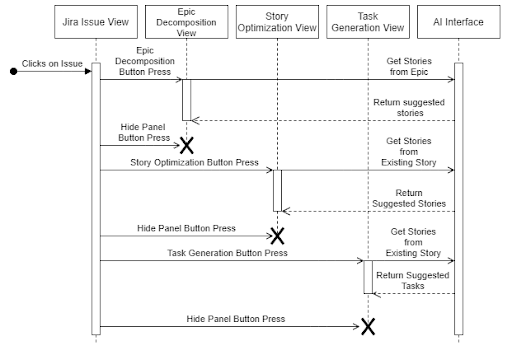
\includegraphics[width=\textwidth,height=\textheight,keepaspectratio]{./figure/SequenceFlowDiagram.png}}
\caption{Suggestion web panel sequence diagram representing the flow of messages between the frontend Jira web page and AI4Agile backend}
\end{figure*}

The plugin communicates from the Jira interface to the backend processes through AJAX calls which are received by Flask. When a web panel is opened for any of the three processes, a message is sent to generate and return the suggestion issues. The Jira panel will function asynchronously with a loading animation appearing until the resulting suggestions are received. Once the results are received, populated in the suggestion box, and the desired suggestions are selected by the user, then a message is sent containing which suggestions to then create within Jira.